\documentclass[class=article, crop=false]{standalone}
\usepackage{graphicx}
\graphicspath{{../Figures}}
\setkeys{Gin}{width=0.9\textwidth}

\usepackage{caption}
\usepackage{subcaption}

\usepackage{amsmath}

\usepackage{cleveref}

\begin{document}

\section{Case results}
\label{sec:case}
One case was tested in which the ROV and USV are initialized at the desired point to hold with a given seastate. There are two variables which have been tested: the length of the wire (and thus the starting depth of the ROV) and the waveheight. Specifically, the ROV's height was tested at 0m (analogous to being stowed), 50m and 100m. 0m was chosen as a baseline, showing the USV's performance when not affected by the drag of the ROV. From the plans for the project at the time of writing, the planned maximum operating depth is 100m, making this a natural second datapoint. 50m was chosen as a midpoint between the two for additional data collection.

Data was gathered by a data collection ROS2 node which collected, worked and plotted the data. The data was collected over a period of 30s. This time period was chosen because it was difficult to have the simulation be stable for a longer period while controlled. Looking at the visual output of the simulation it seemed as if the wire physics did unexpected things and caused the simulation to break. It was possible to collect all the data at 30s intervals however, and the data does give enough information to draw conclusions from.

There were five different wave heights that were used for simulations, 0m to 2m in 0.5m intervals. Looking at the simulation and the results, only the three lowest of these seem reasonable to compare. The vessel tumbled a lot for the higher wave heights and the simulation started being very unstable. When the vessel tumbled, sometimes it also got "wrapped up" in the wire, causing further instability.

\begin{figure}[h]
    \centering
    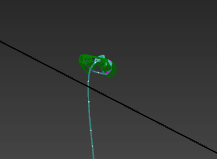
\includegraphics{entwined}
    \caption{Figure showing the USV entwined in the ROV wire due to tumbling in the waves. The vessel is the green wireframe while the tether is the teal and pink line.}
    \label{fig:entwined}
\end{figure}

As mentioned in \cref{chap:cases}, the equation used to simulate the waves is
\[h = 0.5\sin(0.5 x +0.6t) + 0.25\cos(0.6y + 0.3x + 1.45t)\]
Where \(h\) is the height above \(z=0\), \(x\) and \(y\) are the position in the horizontal plane and \(t\) is the time since the simulation started. The shape of this equation can be seen plotted in \cref{fig:wave-shape}

\begin{figure}
    \centering
    \begin{subfigure}{0.45\textwidth}
        \centering
        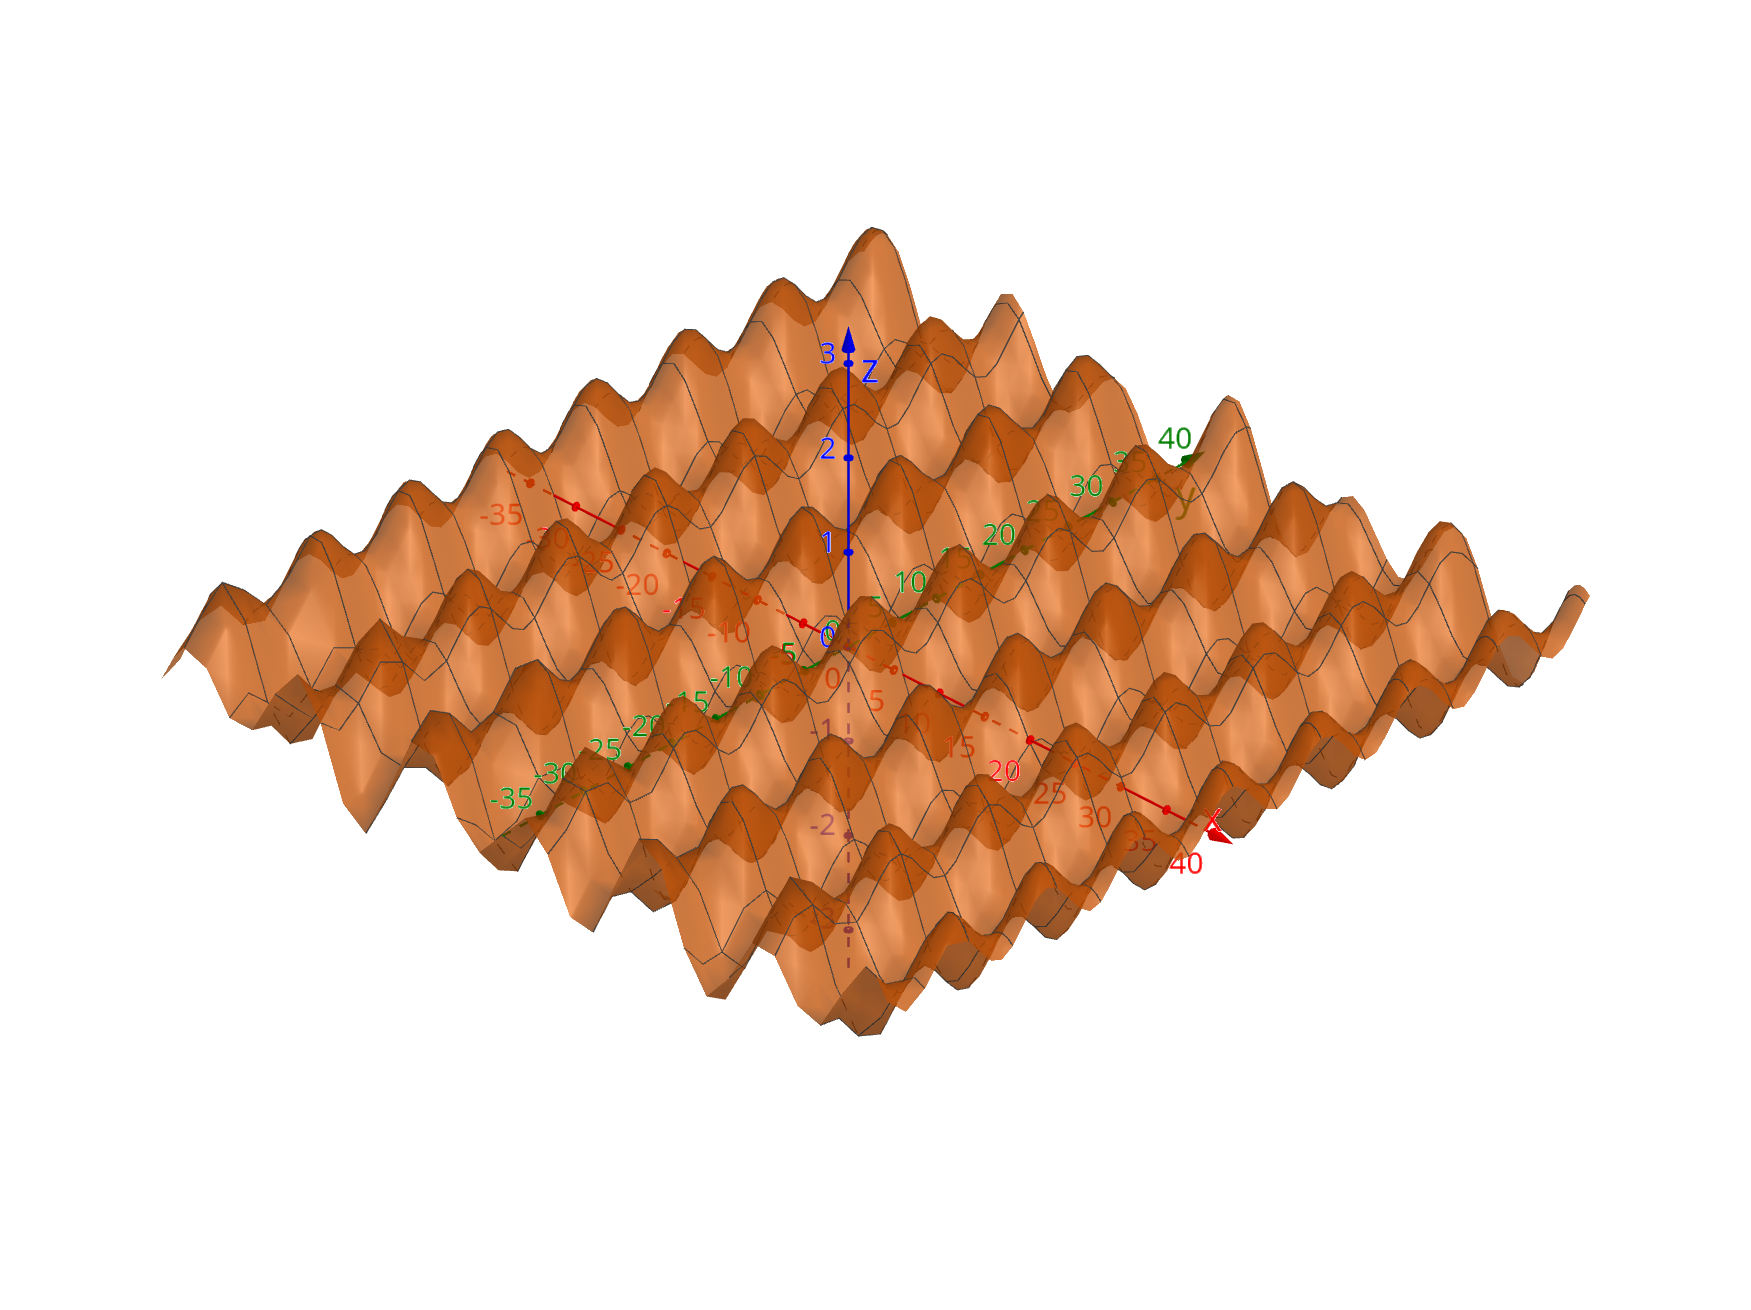
\includegraphics{wave-shape}
        \caption{3D representation. Note that the Z-axis is not scaled the same as the X- and Y-axes}
    \end{subfigure}
    \hfill
    \begin{subfigure}{0.45\textwidth}
        \centering
        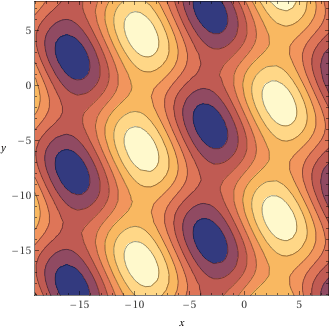
\includegraphics{wave-contour}
        \caption{Contour plot}
    \end{subfigure}
    \caption{The wave-shape for the simulated wave given at \(t=0\).}
    \label{fig:wave-shape}
\end{figure}

A lot of data was collected. Only the data which will be directly discussed in the next chapter will be brought up here. All results can be seen plotted in the appendix \ref{App:data}.

\subsection{Uncontrolled behaviour}
As a baseline, the USV was placed in the simulation with no control system applied. With no waves, as seen in \cref{fig:0-uncontrolled}. Uncontrolled and with higher waves can be seen in \cref{fig:0.5m-uncontrolled} and \cref{fig:1.0m-uncontrolled}. These three figures show the USV's position in X- and Y- direction. The starting position is represented by a dot and the desired position is represented by an X in the plot. The line shows the position the USV follows as time progresses. The results in those three figures are very similar within each group, and so for brevity only one example is shown for each.

\begin{figure}
    \centering
    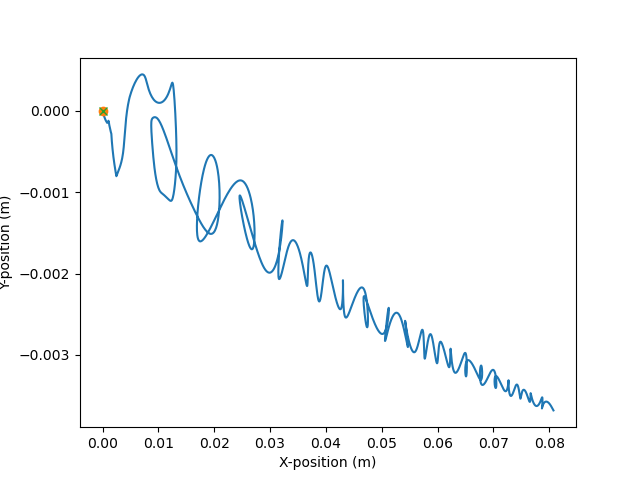
\includegraphics{scenario1/rov-0m/0.0m/usv_position_uncontrolled}
    \caption{The USV's position uncontrolled with 0m waves with the ROV retracted}
    \label{fig:0-uncontrolled}
\end{figure}

\begin{figure}
    \centering
    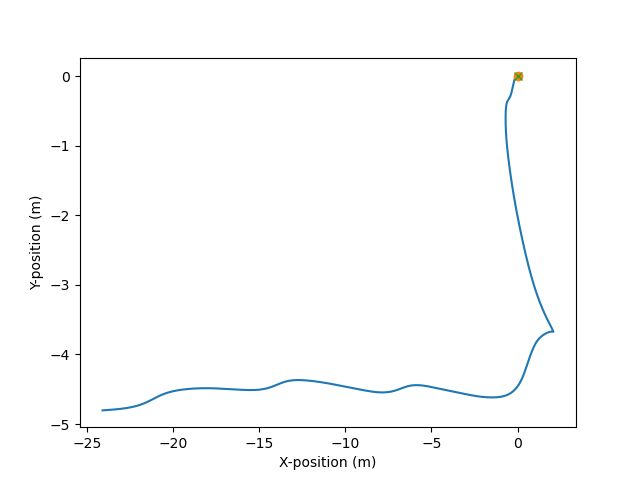
\includegraphics{scenario1/rov-0m/0.5m/usv_position_uncontrolled}
    \caption{The USV's movement uncontrolled with 0.5m waves with the ROV retracted}
    \label{fig:0.5m-uncontrolled}
\end{figure}

\begin{figure}
    \centering
    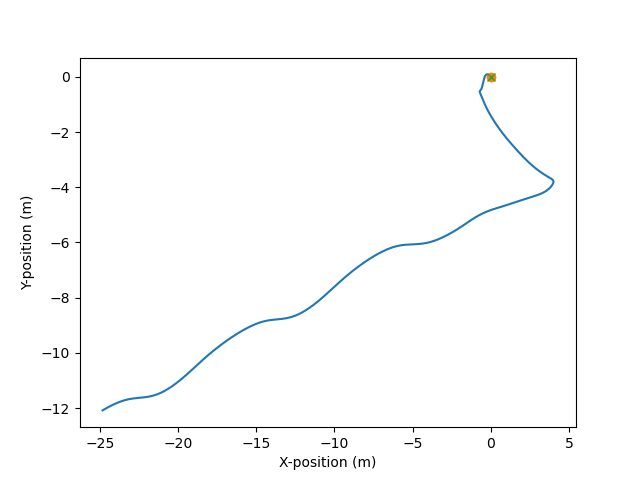
\includegraphics{scenario1/rov-0m/1.0m/usv_position_uncontrolled}
    \caption{The USV's movement uncontrolled with 1m waves with the ROV retracted}
    \label{fig:1.0m-uncontrolled}
\end{figure}

For the 0m wave case there is minimal movement, on the order of millimeters. This is likely due to noise and chaos in the simulation, small initial conditions randomized with time which cause calculations to be slightly different. It is probably safe to ignore the movement in the 0m case. There are similarities between the 0.5m wave height and the 1m wave height cases. There is a movement south-west first before it moves south-east. What likely happens here is that the vessel finds some local minimum in the wave shape and is carried along it. Sadly, the shape of the waves is not visually represented in the simulation in real-time, so this is not visually confirmed. Because of the minimal movement with no wave interference, the 0m wave case will not be further plotted here. It is however plotted fully in the appendix.

The error for the position can be seen in \cref{fig:position_errors}. The various position errors have a similar shape but vary in magnitude. Comparing the error at 0.5m waves with the position at 0.5m waves, \cref{fig:position_errors} and \cref{fig:0.5m-uncontrolled}, it is visible that these results are at least connected. The Y-direction error increases early then is stable, while the X-direction error goes first in one direction and then in the other until the simulation ends. The magnitudes of the results are also comparable and as expected.

\begin{figure}
    \centering
    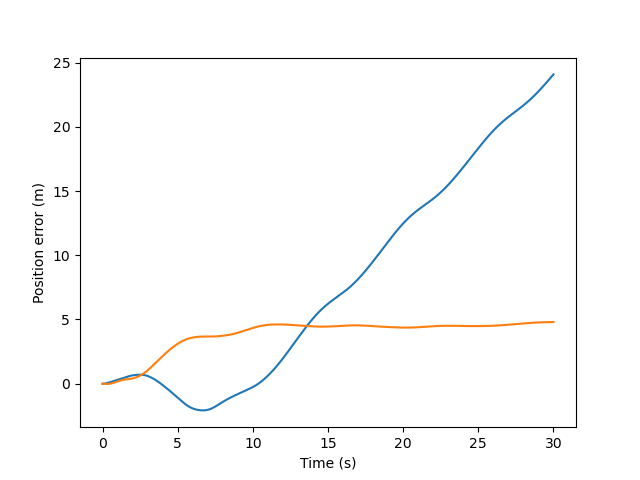
\includegraphics{scenario1/rov-0m/0.5m/usv_pos_error_uncontrolled}
    \caption{The USV's position error, uncontrolled with 0.5m waves with the ROV retracted. The X-direction error is in blue while the Y-direction in yellow.}
    \label{fig:position_errors}
\end{figure}

The heading of the USV is also charted. This can be seen in \cref{fig:0.5m-heading-unc}. Once again, the shapes of the different wave heights and ROV-states are very similar, and so for brevity, only one example will be brought up. The desired heading here is the starting heading, i.e. that the vessel stays facing the way that it started. This heading is 180°, or due south. In the 0.5m and 1m waves it does almost an about face, turning to face almost 30°. All of the uncontrolled heading results show similar results. It is therefore reasonable to assume that this is caused by the hydrodynamic effects of the vessel and it finding a stable state with regards to the seastate.

\begin{figure}
    \centering
    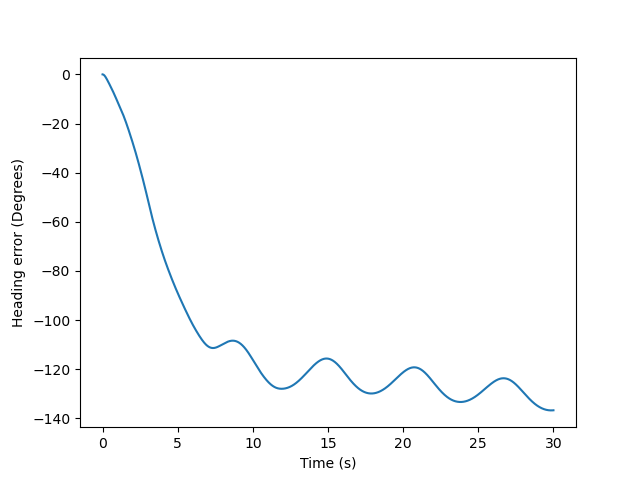
\includegraphics{scenario1/rov-0m/0.5m/usv_heading_error_uncontrolled}
    \caption{The USV's heading uncontrolled with 0.5m waves with the ROV retracted}
    \label{fig:0.5m-heading-unc}
\end{figure}

In this simulation, the ROV is also uncontrolled. With regards to mastering, the USV is defined as the master for this scenario. This means that the ROV's "target position" is directly below the USV. Because of this, the ROV error has also been measured without the control system enabled to use as a control. The position in the horizontal plane can be seen in \cref{fig:rov_xy_error} and the depth error can be seen in \cref{fig:rov_depth_error}. As above, the shapes of the curves are very similar for all cases except the control case, therefore only one example is used. Of note: for some reason the "depth error" plots got some slightly jumbled data in, and therefore plot the "error" as relative to 100m deep. This means that for the ROV at 0m, a value of -100 is desired, for the ROV at 50m, a value of -50 is desired and for the ROV at 100m a value of 0 is desired. This error was spotted too late to remake the plots and thus will be abn error in the depiction.

\begin{figure}
    \centering
    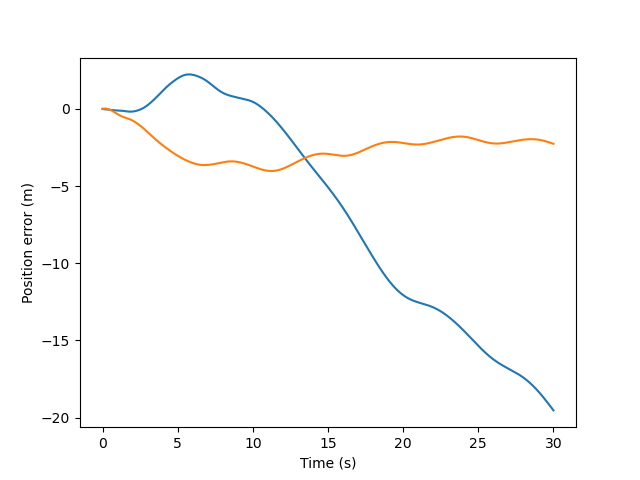
\includegraphics{scenario1/rov-50m/0.5m/rov_position_error_uncontrolled}
    \caption{ROV horizontal error at 50m depth with 0.5m waves}
    \label{fig:rov_xy_error}
\end{figure}

\begin{figure}
    \centering
    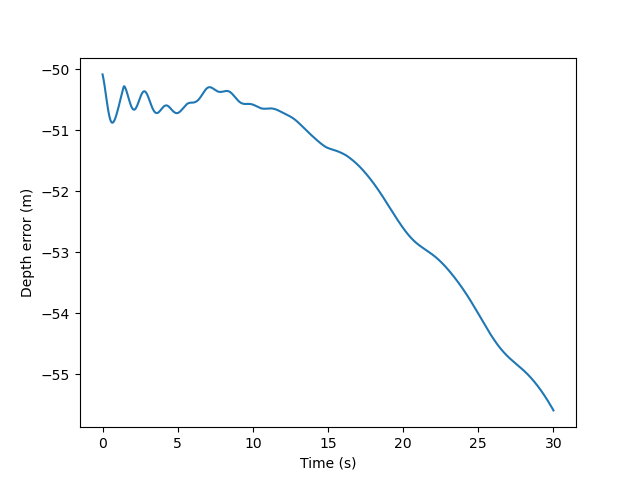
\includegraphics{scenario1/rov-50m/0.5m/rov_depth_error_uncontrolled}
    \caption{ROV depth error at 50m with 0.5m waves. Note the incorrect Y-axis as described in the text.}
\end{figure}



\subsection{Controlled response}
The same simulations as above were performed but this time with the control system enabled. For this scenario, the starting position and target position are the same at \(\begin{bmatrix} 0 & 0 & 0 \end{bmatrix}^T\). In other words, this simulates the vessel being in a stable position and trying to maintain it. In \cref{fig:position-controlled} the movement of the USV can be seen for the ROV at 50m depth. Again, the shape of the results are very similar for the varying ROV depths. The shape of the 1m case (\cref{fig:position_controlled_1m}) is suspiciously close to the uncontrolled case (\cref{fig:fig:1.0m-uncontrolled}). It is not clear whether this is an error in measuring or if 50m is a strange harmonic place. This will be further discussed in the next chapter.

\begin{figure}
    \centering
        \begin{subfigure}{0.8\textwidth}
        \centering
        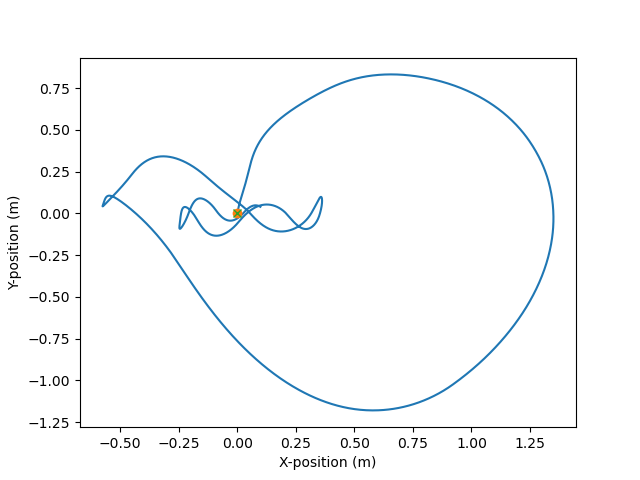
\includegraphics{scenario1/rov-50m/0.0m/usv_position_controlled}
        \caption{0m waves}
    \end{subfigure}
    \vfill
    \begin{subfigure}{0.8\textwidth}
        \centering
        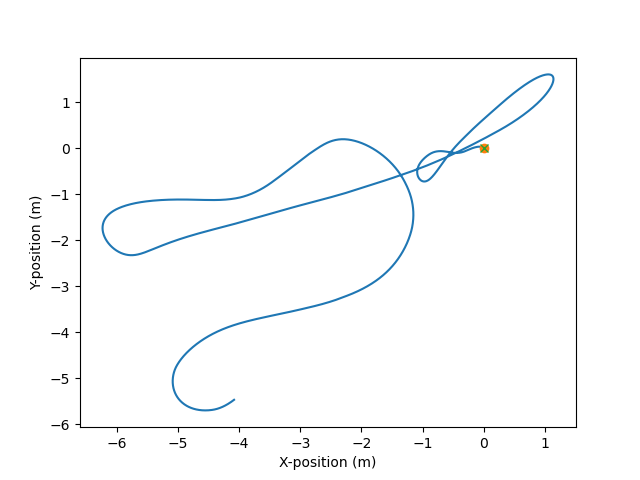
\includegraphics{scenario1/rov-50m/0.5m/usv_position_controlled}
        \caption{0.5m waves}
    \end{subfigure}
    \vfill
        \begin{subfigure}{0.8\textwidth}
        \centering
        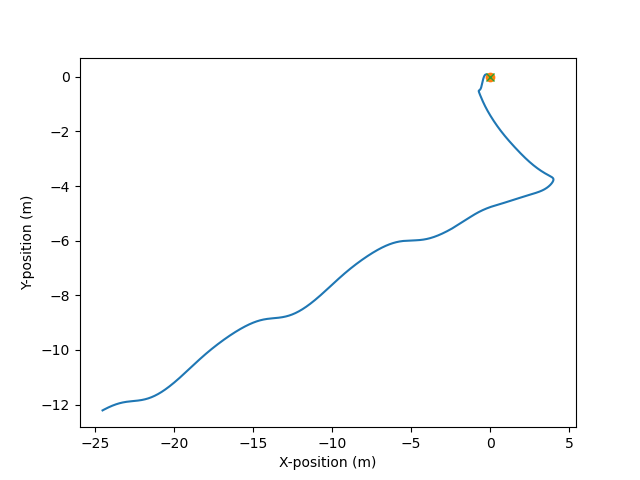
\includegraphics{scenario1/rov-50m/1.0m/usv_position_controlled}
        \caption{1m waves}
        \label{fig:position_controlled_1m}
    \end{subfigure}
    \vfill
    \caption{The USV's movement controlled with varying wave heights, ROV at 50m depth}
    \label{fig:position-controlled}
\end{figure}

The controlled response for the USV position at higher waves demonstrates where a lot of the issues with the simulation come in. This can be seen in \cref{fig:fucked_position} which shows how the control system attempts and struggles to move around.

\begin{figure}
    \centering
    \begin{subfigure}{0.45\textwidth}
        \centering
        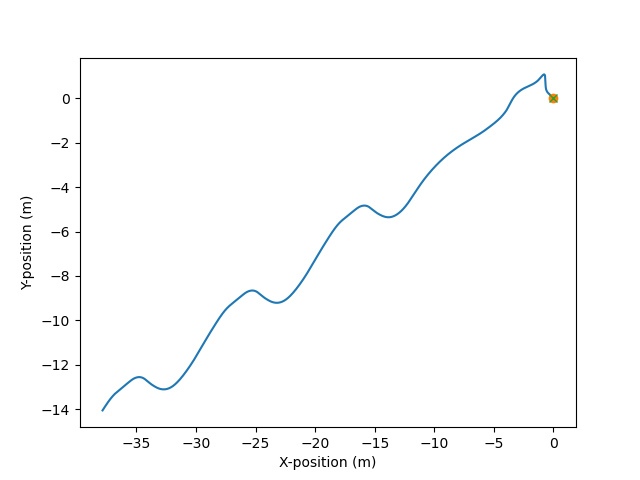
\includegraphics{scenario1/rov-50m/2.0m/usv_position_uncontrolled}
        \caption{Without control}
    \end{subfigure}
    \hfill
    \begin{subfigure}{0.45\textwidth}
        \centering
        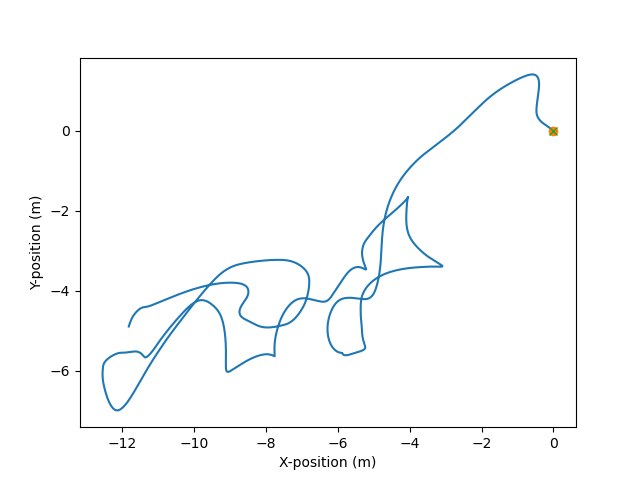
\includegraphics{scenario1/rov-50m/2.0m/usv_position_controlled}
        \caption{With control}
    \end{subfigure}
    \caption{USV position with 2m waves with and without the control system enabled. Notice how "squiggly" the position is in the controlled case}
    \label{fig:fucked_position}
\end{figure}

Similarly, the position error both demonstrates that the control system is working in lower waves (see \cref{fig:position_error_controlled}), but also that it is not working well enough in higher waves, \cref{fig:position_error_controlled_fucked}.

\begin{figure}
    \centering
    \begin{subfigure}{0.45\textwidth}
        \centering
        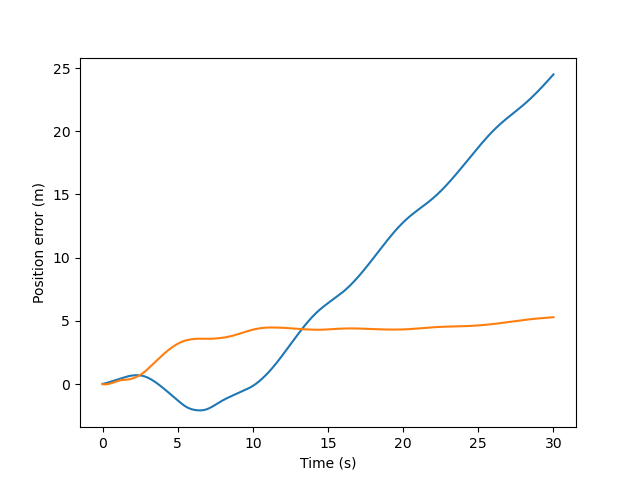
\includegraphics{scenario1/rov-50m/0.5m/usv_pos_error_uncontrolled}
        \caption{Without control}
    \end{subfigure}
    \hfill
    \begin{subfigure}{0.45\textwidth}
        \centering
        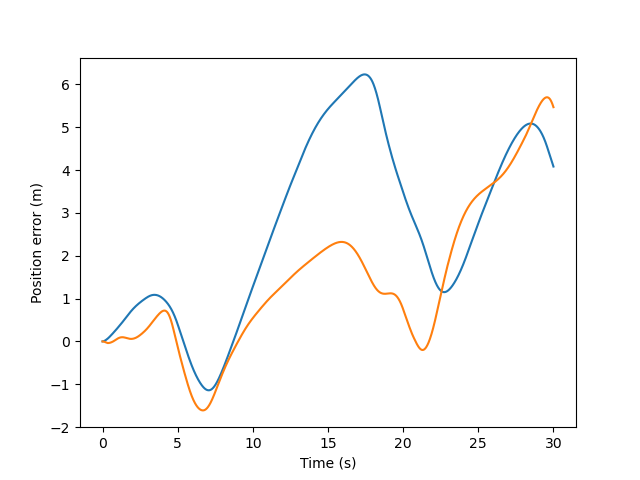
\includegraphics{scenario1/rov-50m/0.5m/usv_pos_error_controlled}
        \caption{With control}
    \end{subfigure}
    \caption{USV position error with 0.5m waves with and without the control system enabled. The amplitude of the error is much lower with control, showing that the control system actually works.}
    \label{fig:position_error_controlled}
\end{figure}

\begin{figure}
    \centering
    \begin{subfigure}{0.45\textwidth}
        \centering
        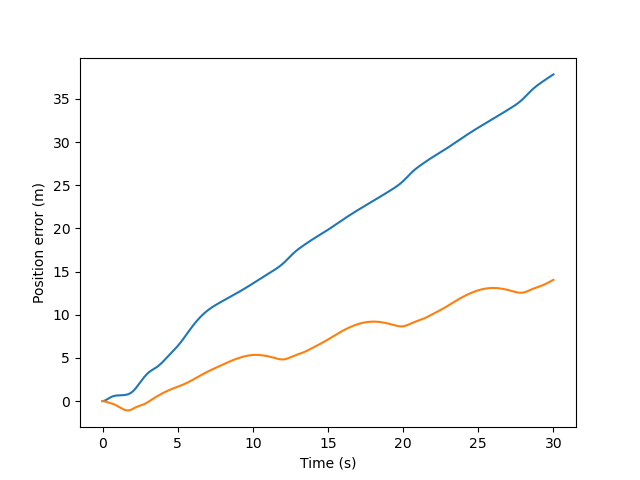
\includegraphics{scenario1/rov-50m/2.0m/usv_pos_error_uncontrolled}
        \caption{Without control}
    \end{subfigure}
    \hfill
    \begin{subfigure}{0.45\textwidth}
        \centering
        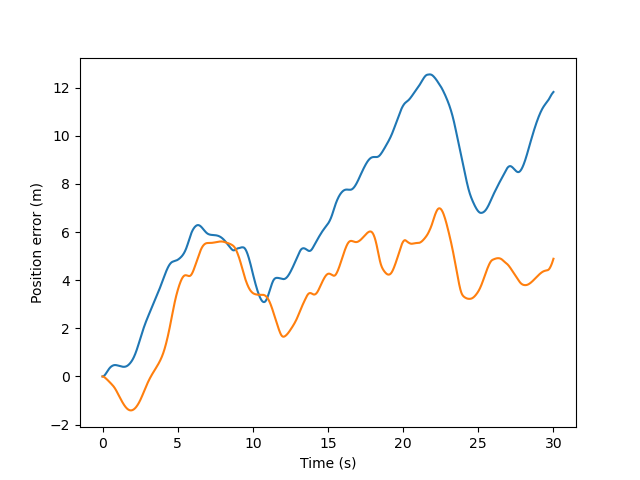
\includegraphics{scenario1/rov-50m/2.0m/usv_pos_error_controlled}
        \caption{With control}
    \end{subfigure}
    \caption{USV position error with 2m waves with and without the control system enabled. The error of the USV is much lower with controls than without}
    \label{fig:position_error_controlled_fucked}
\end{figure}

As for the heading error, the control system seems to be working fairly well. It needs more tuning, but these are promising results. The heading with the ROV deployed to 50m but at different wave heights can be seen in \cref{fig:heading_error_controlled}. The results with the ROV "retracted" had some strange harmonics that can be seen in \cref{fig:heading_swinging}. This is likely due to the swinging mass that is the ROV hanging from underneath the vessel, \cref{fig:ballsack}. Realistically, the ROV would have some sort of launch-and-recovery system that locks it into a more stationary position when retracted and stowed. This would all but eliminate this swinging mass problem, but has not been simulated here.

\begin{figure}
    \centering
    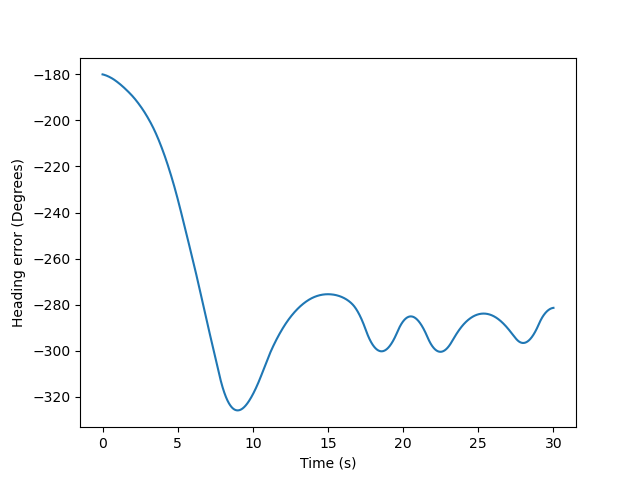
\includegraphics{scenario1/rov-0m/0.0m/usv_heading_error_controlled}
    \caption{Heading error for the USV with the ROV retracted with 0m waves. Notice that the controller is not able to reach the desired set point of 0.}
    \label{fig:heading_swinging}
\end{figure}

The desired heading for this setting is 0°, or due north. Due to the nature of the data being constrained between 0 and -360 (as it is an error), the plotting is in this range as well, this causes some strange shapes to appear as the vessel oscillates about 0. This was attempted fixed but could not be done in time. As such, the shape of \cref{fig:heading_error_0m} is nearly perfect, only having some oscillations but working well. The heading controller has not been tuned very well, and so with more attention paid to tuning it, these results could potentially be improved a lot.

\begin{figure}
    \centering
    \begin{subfigure}{0.65\textwidth}
        \centering
        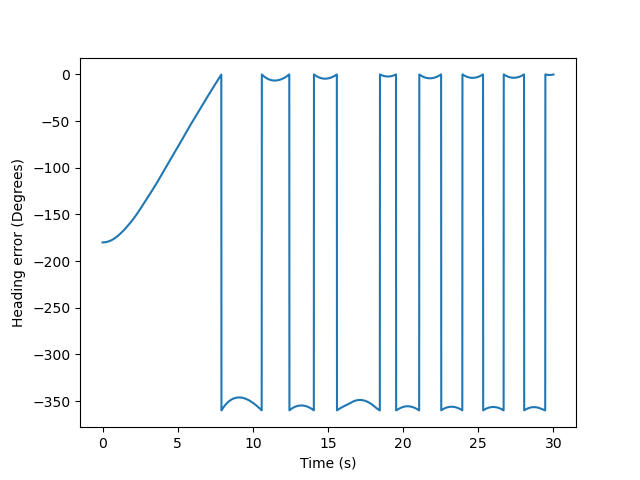
\includegraphics{scenario1/rov-50m/0.0m/usv_heading_error_controlled}
        \caption{0m waves}
        \label{fig:heading_error_0m}
    \end{subfigure}
    \vfill
    \begin{subfigure}{0.65\textwidth}
        \centering
        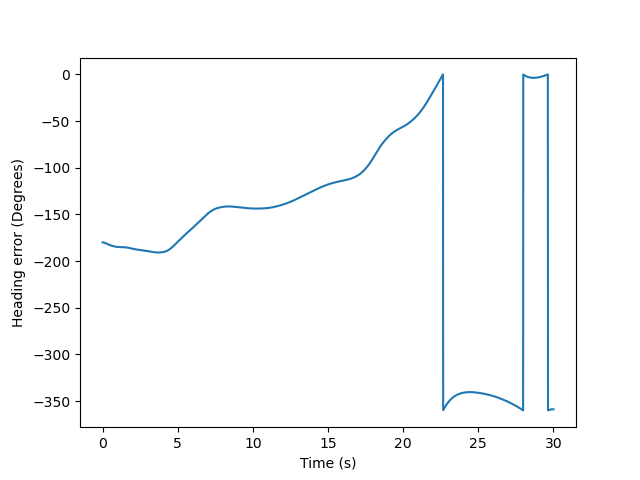
\includegraphics{scenario1/rov-50m/0.5m/usv_heading_error_controlled}
        \caption{0.5m waves}
    \end{subfigure}
    \vfill
    \begin{subfigure}{0.65\textwidth}
        \centering
        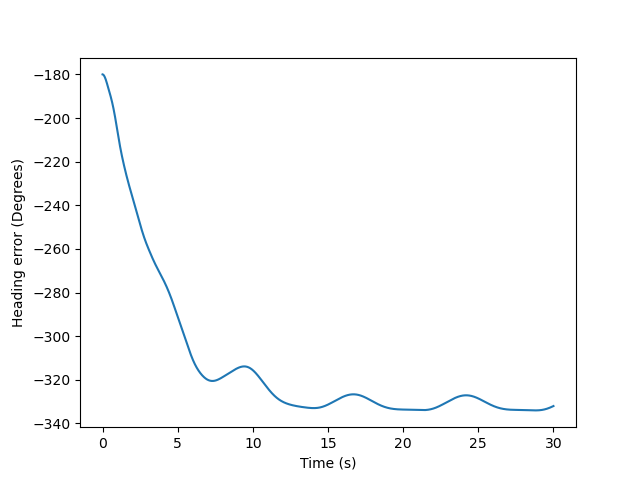
\includegraphics{scenario1/rov-50m/1.0m/usv_heading_error_controlled}
        \caption{1m waves}
        \label{fig:position_controlled_1m}
    \end{subfigure}
    \vfill
    \caption{The USV's heading error with control and varying wave heights, ROV at 50m depth}
    \label{fig:heading_error_controlled}
\end{figure}

In addition to the heading and position data from the uncontrolled cases, in the controlled cases the forces applied by the controller were also recorded. The applied forces are nearly identical for the different ROV depth configurations. Some examples of the lateral forces can be seen in \cref{fig:lateral_forces} while torque can be seen in \cref{fig:torque}. Of note: both the lateral and momentum forces are capped by the controller. This is to simulate the maximum allowable authority or allowed force in that direction. This cap does not seem to be reached for the lateral forces, but the plot makes it very clear that the torque forces are very underpowered as the system is saturated most of the time.

\begin{figure}
    \centering
    \begin{subfigure}{0.65\textwidth}
        \centering
        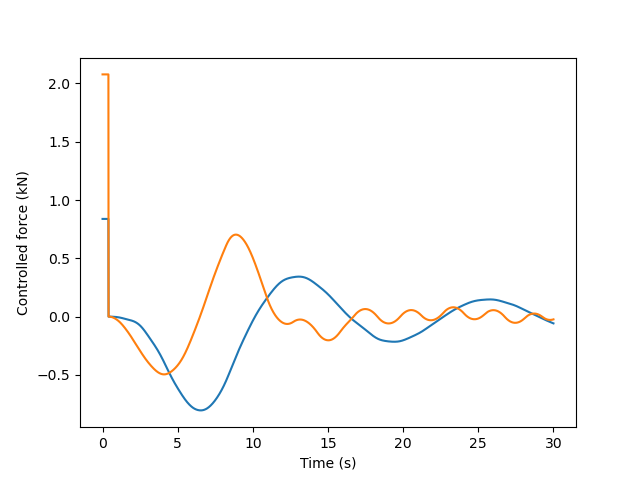
\includegraphics{scenario1/rov-50m/0.0m/usv_forces}
        \caption{0m waves}
    \end{subfigure}
    \vfill
    \begin{subfigure}{0.65\textwidth}
        \centering
        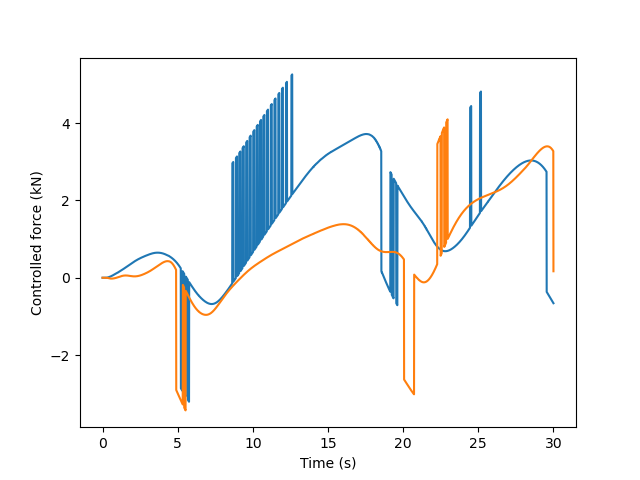
\includegraphics{scenario1/rov-50m/0.5m/usv_forces}
        \caption{0.5m waves}
    \end{subfigure}
    \vfill
    \begin{subfigure}{0.65\textwidth}
        \centering
        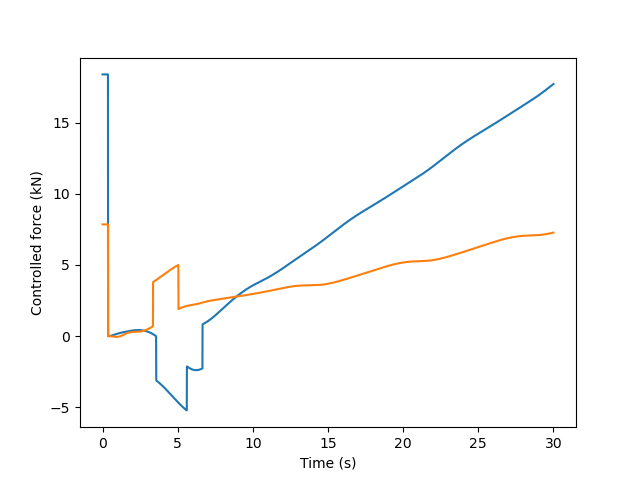
\includegraphics{scenario1/rov-50m/1.0m/usv_forces}
        \caption{1m waves}
        \label{fig:position_controlled_1m}
    \end{subfigure}
    \vfill
    \caption{The USV's lateral forces applied during varying wave heights, ROV at 50m depth}
    \label{fig:lateral_forces}
\end{figure}

Several of the lateral force plots are strangely discontinuous, compare for instance the two plots in \cref{fig:compare_forces}. These are both for the 1m case but with the ROV at different heights. One possibility for the appearance of these discontinuities is the fact that the controllers are currently implemented to take into account the time between steps. This means that if the data collector would wait two ticks before plotting rather than one, the amplitude of the plotted point would be doubled. With natural computation delays in the simulation, this could occur quite frequently.

\begin{figure}
    \centering
    \begin{subfigure}{0.45\textwidth}
        \centering
        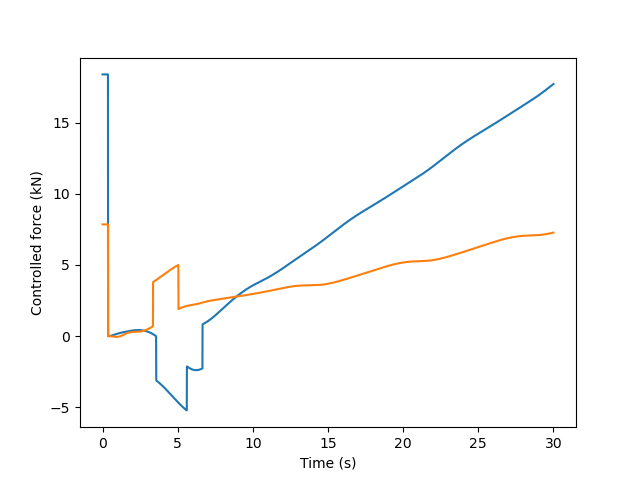
\includegraphics{scenario1/rov-50m/1.0m/usv_forces}
        \caption{ROV at 50m}
    \end{subfigure}
    \hfill
        \begin{subfigure}{0.45\textwidth}
        \centering
        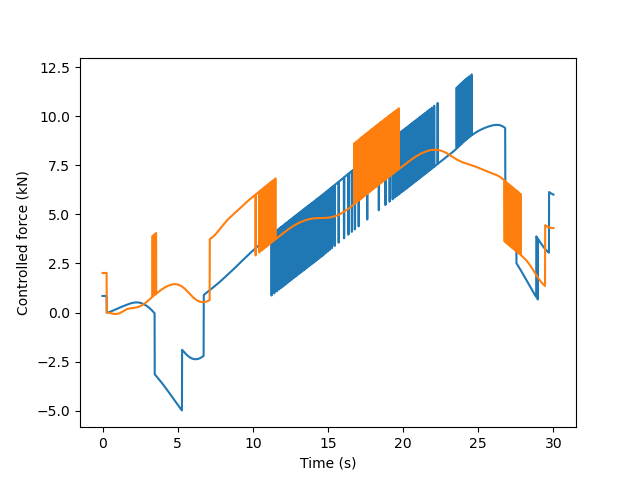
\includegraphics{scenario1/rov-100m/1.0m/usv_forces}
        \caption{ROV at 100m}
    \end{subfigure}
    \caption{The lateral forces output by the controller at 1m wave height. The overall shape of the forces are similar, but the 100m case has many discontinuities while the 50m case does not.}
\end{figure}

\begin{figure}
    \centering
    \begin{subfigure}{0.65\textwidth}
        \centering
        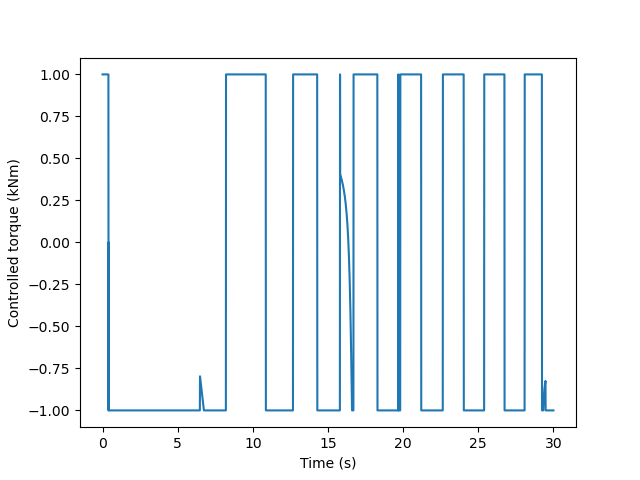
\includegraphics{scenario1/rov-50m/0.0m/usv_torque}
        \caption{0m waves}
    \end{subfigure}
    \vfill
    \begin{subfigure}{0.65\textwidth}
        \centering
        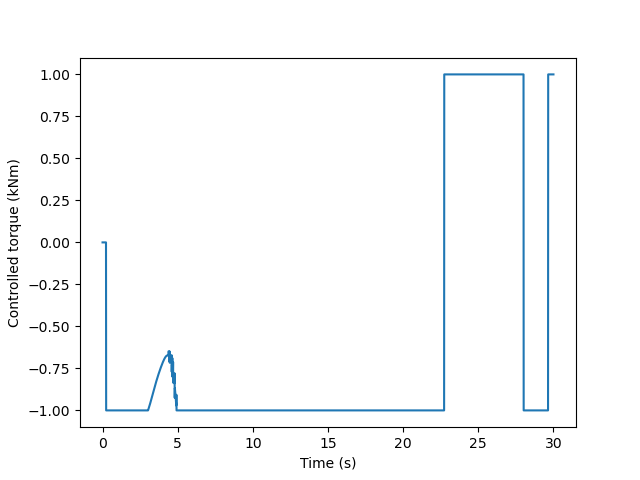
\includegraphics{scenario1/rov-50m/0.5m/usv_torque}
        \caption{0.5m waves}
    \end{subfigure}
    \vfill
    \begin{subfigure}{0.65\textwidth}
        \centering
        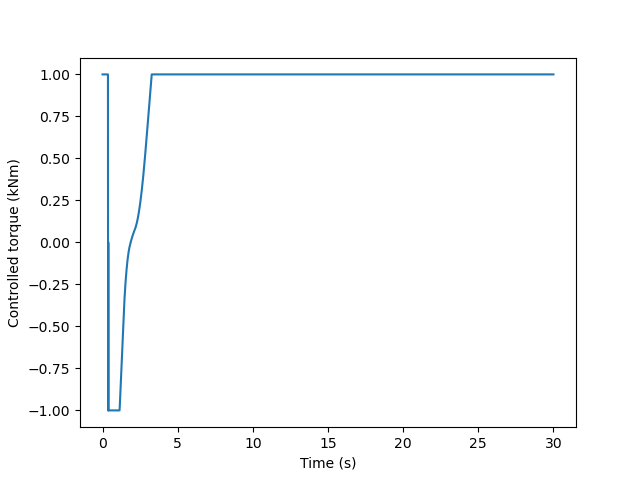
\includegraphics{scenario1/rov-50m/1.0m/usv_torque}
        \caption{1m waves}
        \label{fig:position_controlled_1m}
    \end{subfigure}
    \vfill
    \caption{The USV's torque applied during varying wave heights, ROV at 50m depth. The system is capped at 1kNm of torque and is saturated at this level for most of the time}
    \label{fig:torque}
\end{figure}

The ROV's controller is also tested and shows similar results to above. It is able to keep up when there is no movement or when the waves are low, but when the waves reach and exceed 1m in height the system struggles to keep up. The case for the ROV at 100m at different wave heights can be seen in \cref{fig:rov_position_error_controlled}

\begin{figure}
    \centering
    \begin{subfigure}{0.65\textwidth}
        \centering
        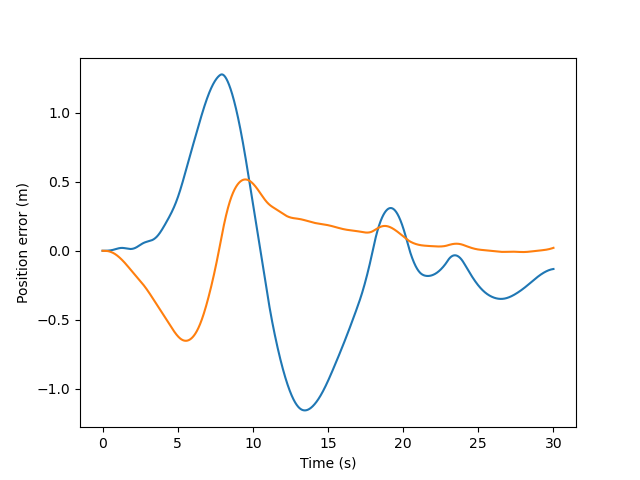
\includegraphics{scenario1/rov-100m/0.0m/rov_position_error_controlled}
        \caption{0m waves}
    \end{subfigure}
    \vfill
    \begin{subfigure}{0.65\textwidth}
        \centering
        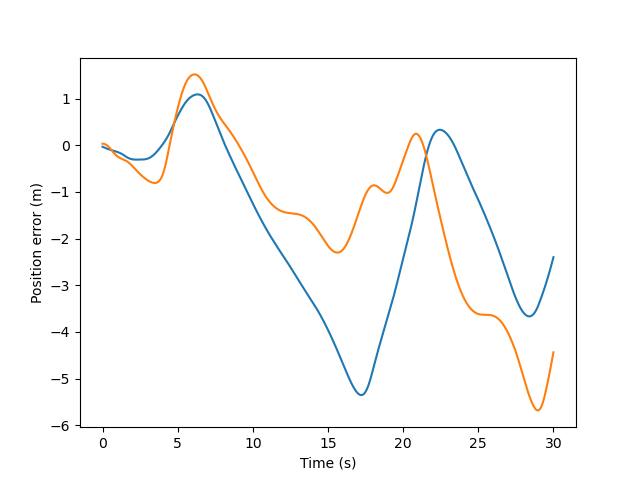
\includegraphics{scenario1/rov-100m/0.5m/rov_position_error_controlled}
        \caption{0.5m waves}
    \end{subfigure}
    \vfill
    \begin{subfigure}{0.65\textwidth}
        \centering
        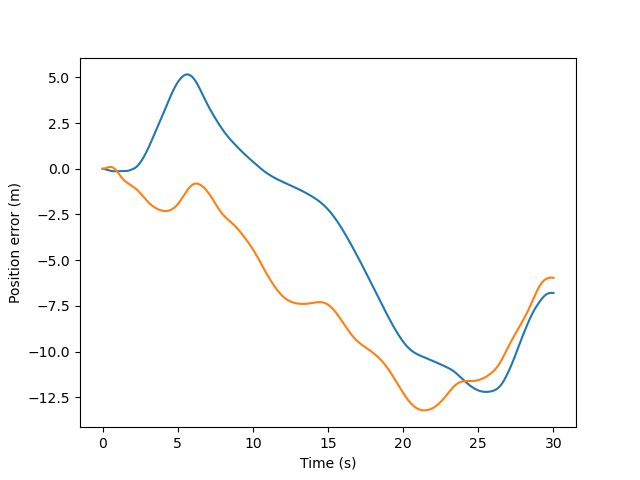
\includegraphics{scenario1/rov-100m/1.0m/rov_position_error_controlled}
        \caption{1m waves}
        \label{fig:position_controlled_1m}
    \end{subfigure}
    \vfill
    \caption{The ROV's positional error in the XY plane at 100m depth with different wave heights.}
    \label{fig:rov_position_error_controlled}
\end{figure}

The depth control needs definite work, but is also capable of holding position. The case at 100m is shown in \cref{fig:rov_depth_error_controlled}. A comparison between a controlled depth and uncontrolled is shown in \cref{fig:depth_comparison}.

\begin{figure}
    \centering
    \begin{subfigure}{0.65\textwidth}
        \centering
        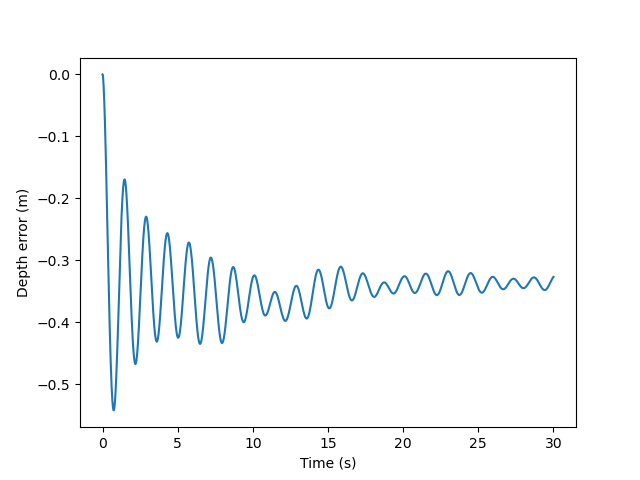
\includegraphics{scenario1/rov-100m/0.0m/rov_depth_error_controlled}
        \caption{0m waves}
    \end{subfigure}
    \vfill
    \begin{subfigure}{0.65\textwidth}
        \centering
        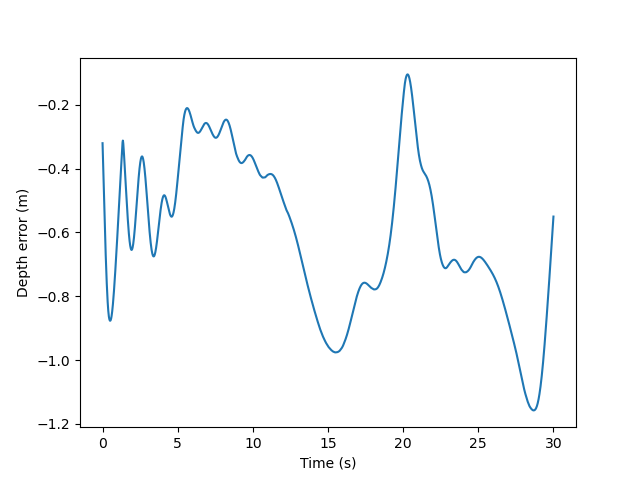
\includegraphics{scenario1/rov-100m/0.5m/rov_depth_error_controlled}
        \caption{0.5m waves}
    \end{subfigure}
    \vfill
    \begin{subfigure}{0.65\textwidth}
        \centering
        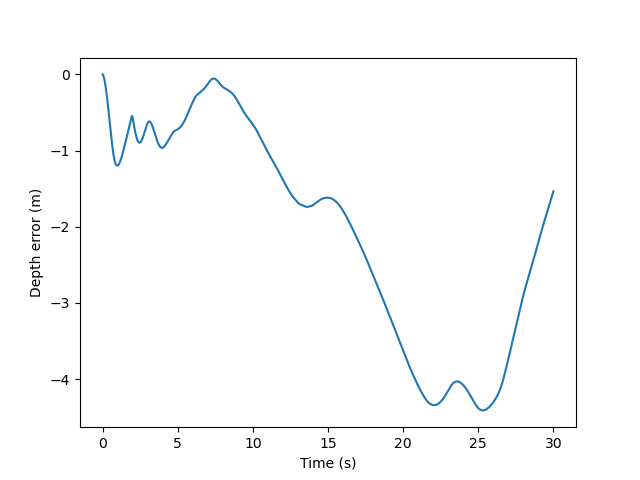
\includegraphics{scenario1/rov-100m/1.0m/rov_depth_error_controlled}
        \caption{1m waves}
        \label{fig:position_controlled_1m}
    \end{subfigure}
    \vfill
    \caption{The ROV's depth error at 100m depth with different wave heights.}
    \label{fig:rov_depth_error_controlled}
\end{figure}

\begin{figure}
    \centering
    \begin{subfigure}{0.8\textwidth}
        \centering
        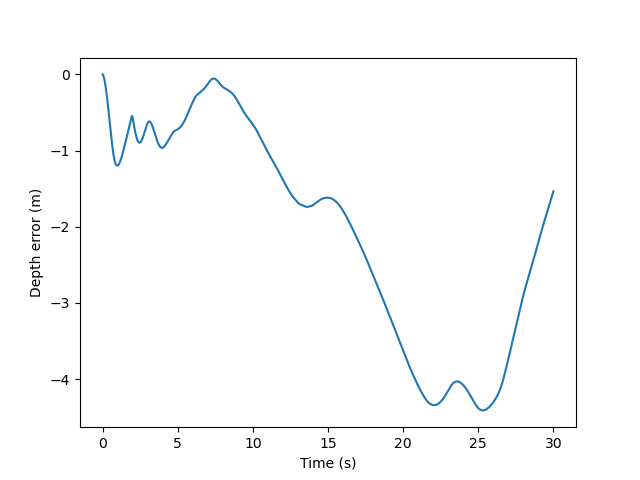
\includegraphics{scenario1/rov-100m/1.0m/rov_depth_error_controlled}
        \caption{With control}
    \end{subfigure}
    \vfill
    \begin{subfigure}{0.8\textwidth}
        \centering
        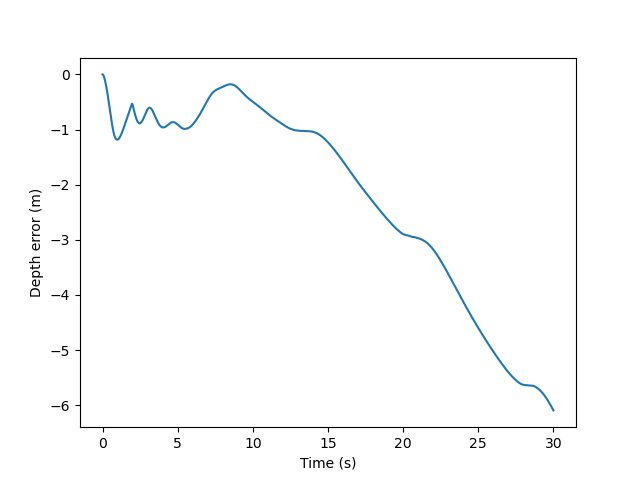
\includegraphics{scenario1/rov-100m/1.0m/rov_depth_error_uncontrolled}
        \caption{Without control}
    \end{subfigure}
    \caption{Comparison of ROV depth error at 100m depth and 1m wave height between a controlled and uncontrolled system. Note that the magnitude of error is almost twice as high for the uncontrolled system.}
    \label{fig:depth_comparison}
\end{figure}

\section{Simulator results}
As mentioned in previous chapters, the simulation was a continued work based on a specialization project which was undertaken in the fall semester of 2024, \cref{specialization}. The goal of the simulation was to provide an environment for tuning and development of the control system. As such, using the commercially available simulation framework AGX Dynamics, developed by Algoryx AB was seen as reasonable.

AGX Dynamics is used as a simulation framework for both machine-in-the-loop systems as well as for simulation of dynamic systems including wires, granulates and hydrodynamic/aerodynamic situations. The reasoning has been that if it's good enough for these purposes it will be good enough for this project.

\subsection{Validation}
Validation of the simulator was primarily performed in the specialization project. \cref{specialization}, section 4.2. There it was done as both an imperical measurement as well as a more general measurement. The specialization project found that the simulator performs as expected.

As a summary of the validation, the tension experienced by the tether between the ROV and the USV was both calculated using manual methods and simulated. The calculations and simulations were performed at 6 different speeds, between 0m/s and 5m/s in 1m/s increments. The ROV was observed in the simulations to drag behind the USV, since the USV is the powered part in this validation and the ROV is only hanging behind as a passive part. As the angle of the tether changes, the cross-sectional area of the ROV as well as the drag coefficient changes. To account for this, the calculated drag was calculated at two separate drag coefficients, one for a flat-facing cuboid and one for an edge-facing cuboid, respectively chosen from tables as 2.05 and 1.05. The forward facing area was assumed in calculations to be constant, however this is an obvious simplification and source of error.

The tension calculated on the wire was compared to the tension provided by the simulator, and was found to be within an acceptable range of error. The deviation between calculation and simulation was found to be between 3\% and 55\%, which considering the severe simplifications assumed makes the results of the simulation seem valid. Additionally, as could be expected, the deviation between calculation and simulation changes as the speed, and thus the drag coefficient and forward facing area, changes. At low speeds, the lower drag coefficient provides more accurate results, while at higher speeds the higher drag coefficient provides more accurate results. This is likely an effect of the forward facing area changing significantly, but is consistent with the expectation looking at the simulation, that the drag increases with speed. Accounting for this change in drag with speed, the deviation can be said to be between 3\% and 20\%, which is definitely within acceptable ranges for accuracy.

All these elements are discussed further and in greater detail in section 4 of the specialization project.

\subsection{Developments of the simulation}
A few developments have been made to the simulation itself. Primarily when it comes to ease of use. The largest change is the move from the controller being embedded in the simulator script to the simulator and controller being two different scripts. This has also allowed the previously monolithic "controller", which handled both position estimation, force calculation, the control loop itself and feedback, to be split into several smaller components that are easier to trouble-shoot, develop and exchange if necessary.

The new controller architecture has already been discussed somewhat and shown in \cref{fig:control-system}. All the elements that are shown in the figure have been developed, but the allocator has been disabled due to issues with trouble-shooting it.

Another development is a further refinement of the wave simulation. Previously it was a choice of waves on or off, but now the waves can be assigned a specific wave height. This allows for the kind of simulations that have been described above.
\end{document}
